%versi 2 (8-10-2016)-pppppppppppppp;
\chapter{Perancangan dan Implementasi}
\label{chap:perancanganDanImplementasi}
\setcounter{secnumdepth}{3}

\paragraph{}
\section{Perancangan Basis Data}
\subsection{Diagram Hubungan Entitas}
Dari analisis yang telah dilakukan, maka dibuatlah Diagram Hubungan Entitas seperti pada gambar 4.1

\begin{figure} [H]
	\centering  
	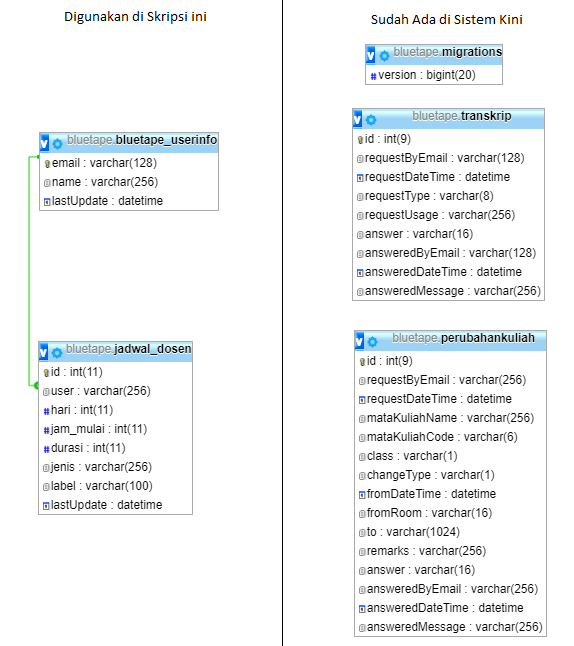
\includegraphics[scale=0.9]{ERDiagram.png}  
	\caption[Diagram Hubungan Entitas]{Diagram Hubungan Entitas} 
	\label{fig:skematik-phpexcel} 
\end{figure}

\subsection{Perancangan Tabel}
\begin{center}
	\begin{table}[H]
	\begin{tabular}{|c|c|c|c|c|c|}
 			\hline
		\textbf{Atribut} & \textbf{Tipe Data} & \textbf{Ukuran} & \textbf{PK* / FK*}  & \textbf{Keterangan} \\
			\hline
		 id & int & 11 & PK &  id jadwal\\
			 \hline
			 user & varchar & 256 & FK &   pemilik jadwal\\
			 \hline
			 hari & int & 11 & bukan keduanya &   hari berlangsungnya jadwal\\
			 \hline
			 jam\_mulai & int & 11 & bukan keduanya &  jam berlangsungnya jadwal\\
			 \hline
			 durasi & int & 11 & bukan keduanya &  lama jadwal berlangsung\\
			 \hline
			 jenis & varchar & 256 & bukan keduanya &  jenis kegiatan jadwal\\
			 \hline
			 label & varchar & 256 & bukan keduanya &   nama kegiatan\\
			 \hline
	\end{tabular}
	\caption{Perancangan Tabel jadwal\_dosen}
	\end{table}
\end{center}
\textit{*PK = Primary Key} \\
Keterangan atribut:
	\begin{enumerate}
		\item \textbf{id}: sebagai penanda yang membedakan setiap jadwal satu sama lain. Memiliki \textit{length default} int dari MySQL yaitu 11. Merupakan \textit{primary key} karena id harus unik agar setiap jadwal dapat dibedakan.
		\item \textbf{user}: email pemilik jadwal. \textit{Foreign key }ini memiliki referensi ke atribut \textit{email} di tabel bluetape\_userinfo. Merupakan \textit{foreign key} untuk mendapatkan data-data milik pengguna.
		\item \textbf{hari}: hari berlangsungnya jadwal. Nilai 0 menandakan hari Senin, 1 hari Selasa, 2 hari Rabu, 3 hari Kamis dan 4 haru Jumat.  Memiliki \textit{length default} int dari MySQL yaitu 11.
		\item \textbf{durasi}: lama berlangsungnya jadwal dalam satuan jam dengan durasi minimal 1 jam.  Memiliki \textit{length default} int dari MySQL yaitu 11.
		\item \textbf{jenis}: jenis kegiatan jadwal. Menggunakan varchar untuk mengantisipasi penambahan fitur pengguna dapat menambahkan jenis kegiatan sendiri.
		\item \textbf{label}: nama kegiatan jadwal. Menggunakan varchar karena nama label diisi oleh pengguna.
	\end{enumerate}

\subsection{Perancangan Rinci}
\subsubsection{Controller EntriJadwalDosen}
\paragraph{} Berikut adalah perancangan kelas Controller EntriJadwalDosen \\
\begin{center}
	\begin{table}[H]
\begin{tabular}{|c|p{11cm}|}
\hline
Nama Method 	& 	insert 	\\
\hline
Parameter Input & data\_jadwal[] via POST \\
\hline
Parameter Output & redirect base\_URL/EntriJadwalDosen\\
\hline
Tabel yang berhubungan & jadwal\_dosen \\
\hline
Deskripsi	& Proses untuk memasukan jadwal \\
\hline
Algoritma	& \begin{itemize}
				\item proses menerima input-input data dari user
				\item proses mengecek apakah data-data yang dimasukan sudah valid
				\item proses mengecek apakah jadwal yang bertabrakan dengan jadwal lain atau tidak
				\item bila jadwal bertabrakan dengan jadwal lain maka proses menampilkan pesan "Jadwal gagal dimasukan. Sudah ada jadwal lain pada waktu ini"
				\item bila tidak ada masalah, proses akan memasukan data ke dalam database
				\end{itemize} \\
\hline
\end{tabular}
\caption{Perincian method insert}
\end{table}
\end{center}

\begin{center}
\begin{table}[H]
\begin{tabular}{|c|p{11cm}|}
\hline
Nama Method 	& 	edit 	\\
\hline
Parameter Input & id\_jadwal,data\_jadwal[] via POST \\
\hline
Parameter Output & redirect base\_URL/EntriJadwalDosen \\
\hline
Tabel yang berhubungan & jadwal\_dosen \\
\hline
Deskripsi	& Proses untuk mengubah jadwal yang sudah dimasukan sebelumnya \\
\hline
Algoritma	& \begin{itemize}
				\item proses menerima input-input data dari user
				\item proses mengecek apakah data-data yang dimasukan sudah valid
				\item proses mengecek apakah waktu baru dari jadwal yang diubah bertabrakan dengan jadwal lain atau tidak
				\item bila jadwal bertabrakan dengan jadwal lain maka proses menampilkan pesan "Pengubahan gagal. Sudah ada jadwal lain pada waktu ini"
				\item bila tidak ada masalah, maka jadwal akan memperbarui data yang ada di database.
				\end{itemize} \\
\hline
\end{tabular}
\caption{Perincian method edit}
\end{table}
\end{center}

\begin{center}
\begin{table}[H]
\begin{tabular}{|c|p{11cm}|}
\hline
Nama Method 	& 	delete 	\\
\hline
Parameter Input & id\_jadwal via POST \\
\hline
Parameter Output & redirect base\_URL/EntriJadwalDosen \\
\hline
Tabel yang berhubungan & jadwal\_dosen \\
\hline
Deskripsi	& Proses untuk menghapus jadwal \\
\hline
Algoritma	& \begin{itemize}
				\item proses menerima pilihan jadwal yang akan dihapus oleh user.
				\item proses mengeluarkan form konfirmasi untuk memastikan user untuk menghapus jadwal yang bersangkutan
				\item bila user memilih "ya", maka data jadwal yang bersangkutan akan dihapus dari database.
				\item bila pilihan user "tidak" maka proses akan menampilkan halaman sebelum user menekan tombol \textit{delete}.
				\end{itemize} \\
\hline
\end{tabular}
\caption{Perincian method \textit{delete}}
\end{table}
\end{center}


\subsubsection{Controller LihatJadwalDosen}
\paragraph{} Berikut adalah perincian rancangan kelas Controller LihatJadwalDosen \\
\begin{center}
\begin{table}[H]
\begin{tabular}{|c|p{11cm}|}
\hline
Nama Method 	& 	index 	\\
\hline
Parameter Input & - \\
\hline
Parameter Output & menampilkan semua jadwal dalam bentuk tabel \\
\hline
Tabel yang berhubungan & jadwal\_dosen \\
\hline
Deskripsi	& Proses untuk memperlihatkan jadwal ke user \\
\hline
Algoritma	& \begin{itemize}
				\item proses memuat semua data jadwal dari database.
				\item proses mengelompokan jadwal-jadwal dari database tersebut berdasarkan pemiliknya.
				\item proses membuat tab-tab setiap tab diberi nama dosen yang sudah memasukan jadwal ke dalam sistem
				\item proses memasukan setiap jadwal yang sudah dipisahkan berdasarkan pemilik ke dalam tab-tab sesuai dengan nama pemilik yang bersangkutan.
				\item secara default akan ditampilkan jadwal dosen yang pertama kali dimuat oleh proses.
				\item bila user menekan tab, proses akan menampilkan semua jadwal dosen terkait
				\end{itemize} \\
\hline
\end{tabular}
\caption{Perincian method index}
\end{table}
\end{center}


\begin{center}
\begin{table}[H]
\begin{tabular}{|c|p{11cm}|}
\hline
Nama Method 	& 	ekspor 	\\
\hline
Parameter Input & - \\
\hline
Parameter Output & file .xls , redirect base\_URL/LihatJadwalDosen \\
\hline
Tabel yang berhubungan & jadwal\_dosen \\
\hline
Deskripsi	& Proses untuk mengkonversi jadwal dari php ke dalam tipe file .xls \\
\hline
Algoritma	& \begin{itemize}
				\item proses memuat semua data jadwal dari database.
				\item proses mengelompokan jadwal-jadwal dari database tersebut berdasarkan pemiliknya.
				\item proses membuat tab-tab di dalam spreadsheet setiap tab diberi nama dosen yang sudah memasukan jadwal ke dalam sistem
				\item proses memasukan setiap jadwal yang sudah dipisahkan berdasarkan pemilik ke dalam tab-tab di speradsheet sesuai dengan nama pemilik yang bersangkutan.
				\item secara default akan ditampilkan jadwal dosen yang pertama kali dimuat oleh proses.
				\item bila user menekan tab, proses akan menampilkan semua jadwal dosen terkait
				\end{itemize} \\
\hline
\end{tabular}
\caption{Perincian method ekspor}
\end{table}
\end{center}


\subsubsection{Model JadwalDosen}
\paragraph{} Berikut adalah perincian rancangan kelas Model JadwalDosen

\begin{center}
\begin{table}[H]
\begin{tabular}{|c|p{11cm}|}
\hline
Nama Method 	& 	add\_jadwal 	\\
\hline
Parameter Input & data\_jadwal[] via POST \\
\hline
Parameter Output & data jadwal ditambahkan ke database \\
\hline
Tabel yang berhubungan & jadwal\_dosen \\
\hline
Deskripsi	& Proses untuk memasukan jadwal ke dalam \textit{database} \\
\hline
Algoritma	& \begin{itemize}
				\item proses menerima data dari user
				\item data-data dimasukan ke dalam \textit{database}
				\end{itemize} \\
\hline
\end{tabular}
\caption{Perincian method add\_jadwal}
\end{table}
\end{center}


\begin{center}
\begin{table}[H]
\begin{tabular}{|c|p{11cm}|}
\hline
Nama Method 	& 	update\_jadwal 	\\
\hline
Parameter Input & id\_jadwal, data\_jadwal[] via POST \\
\hline
Parameter Output & memperbarui data jadwal di database berdasarkan id \\
\hline
Tabel yang berhubungan & jadwal\_dosen \\
\hline
Deskripsi	& Proses untuk mengupdate data jadwal di \textit{database} berdasarkan pilihan user\\
\hline
Algoritma	& \begin{itemize}
				\item proses menerima data dan id\_jadwal
				\item proses mengupdate data di \textit{database} berdasarkan id\_jadwal
				\end{itemize} \\
\hline
\end{tabular}
\caption{Perincian method update\_jadwal}
\end{table}
\end{center}


\begin{center}
\begin{table}[H]
\begin{tabular}{|c|p{11cm}|}
\hline
Nama Method 	& 	delete\_jadwal 	\\
\hline
Parameter Input & id\_jadwal via POST \\
\hline
Parameter Output & data jadwal di database dihapus berdasarkan id \\
\hline
Tabel yang berhubungan & jadwal\_dosen \\
\hline
Deskripsi	& Proses untuk menghapus data jadwal dari \textit{database} berdasarkan pilihan user \\
\hline
Algoritma	& \begin{itemize}
				\item proses menerima id\_jadwal
				\item prose menghapus data jadwal di database berdasarkan id\_jadwal
				\end{itemize} \\
\hline
\end{tabular}
\caption{Perincian method delete\_jadwal}
\end{table}
\end{center}


\begin{center}
\begin{table}[H]
\begin{tabular}{|c|p{11cm}|}
\hline
Nama Method 	& 	get\_jadwal 	\\
\hline
Parameter Input &  - \\
\hline
Parameter Output & seluruh data jadwal \\
\hline
Tabel yang berhubungan & jadwal\_dosen \\
\hline
Deskripsi	& Proses untuk mengambil semua data jadwal \\
\hline
Algoritma	& \begin{itemize}
				\item proses memuat semua data jadwal dari database.
				\item proses mengirim semua data yang suda dimuat ke controller pemanggil
				\end{itemize} \\
\hline
\end{tabular}
\caption{Perincian method get\_jadwal}
\end{table}
\end{center}


\section{Perancangan Antarmuka}
Pada bagian ini akan dibahas rancangan antarmuka Aplikasi Pembangkit Jadwal Dosen.

\subsection{Perancangan Antarmuka Entri Jadwal Dosen}
Perancangan tamnpilan untuk modul Entri Jadwal Dosen dapat dilihat pada gambar di bawah ini
\begin{figure} [H]
	\centering  
	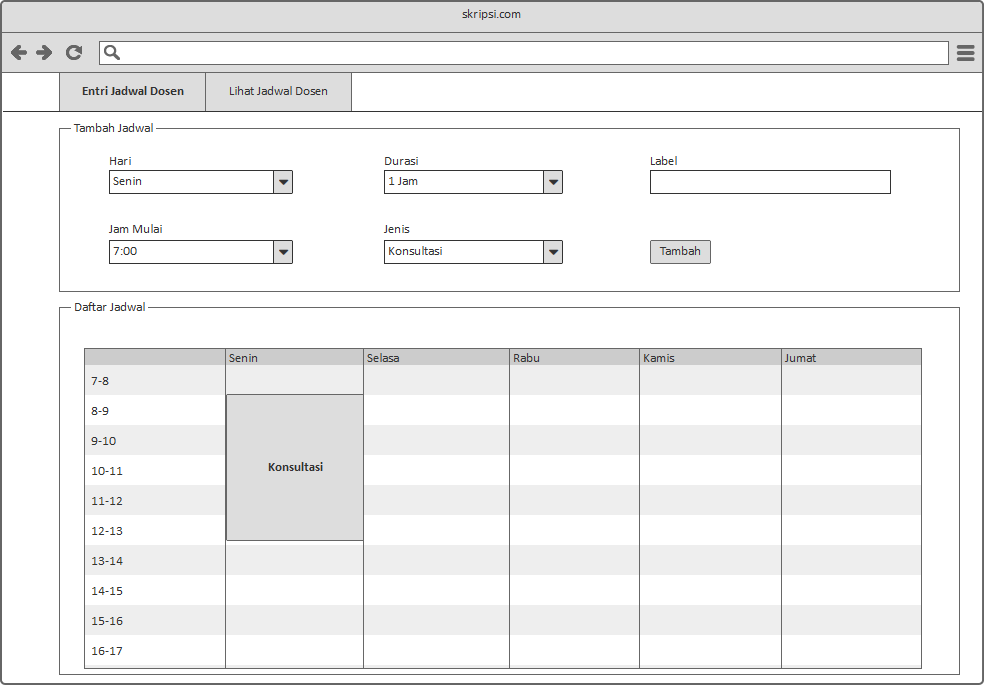
\includegraphics[scale=0.48]{entriJadwalDosen.png}
	\caption[Perancangan Antarmuka Entri Jadwal Dosen]{Perancangan Antarmuka Entri Jadwal Dosen} 
	\label{fig:flow-chart-CodeIgniter} 
\end{figure}
\textbf{Keterangan}
\begin{enumerate}
\item \textbf{Menu Tambah Jadwal}\\ Menu ini berisi field-field yang dapat digunakan pengguna untuk menentukan berbagai macam hal mengenai jadwal yang akan dimasukan sepeti jam dimulainya jadwal, durasi dan lain-lain.
	\begin{itemize}
		\item field Hari: berisi pilihan hari-hari berlangsungnya jadwal. Ada 5 pilihan hari yaitu hari senin, selasa, rabu, kamis, dan jumat.
		\item field Jam Mulai: berisi pilihan jam berlangsungnya jadwal. Jam yang dapat dipilih adalah jam 8 sampai jam 16 (jam 4 sore) dan semua 		pilihan jam tepat pada menit 0, tidak ada pilihan menitnya.
		\item field Durasi: berisi pilihan lama berlangsungnya jadwal. Ada 10 pilihan mulai dari 1 jam, 2 jam, 3 jam dan seterusnya sampai 10 			jam. Sama seperti field Jam Mulai di pilihan ini juga tidak ada pilihan menit.
		\item field Jenis: berisi pilihan jenis kegiatan jadwalnya. Ada 3 pilihan yaitu Konsultasi, Terjadwal dan Kelas.
		\item field Label: diisi dengan nama kegiatan jadwal. Field ini dapat dikosongkan.
		\item tombol Tambah: bila pengguna menekan tombol ini, maka jadwal baru akan ditambahkan sesuai dengan input yang sudah dipilih atau dimasukan oleh pengguna pada field-field di atas.
	\end{itemize}
\item \textbf{Menu Daftar Jadwal} \newline
Tabel pada menu in merepresentasikan hari dan jam perkuliahan. Bila pada jam tertentu ada suatu jadwal, maka sel-sel di yang berada di antara sel jam mulai sampai sel berakhirnya jadwal akan diwarnai sesuai dengan jenis kegiatan jadwalnya. Jadwal konsultasi akan diwarnai hijau, kelas diwarnai putih dan jadwal lainnya yang terjadwal akan diwarnai kuning. Selain itu ditengah-tengah sel yang diwarnai juga akan ditampilkan nama kegiatan jadwalnya yang sudah pengguna isi pada field Label. Contoh tampilan jadwal ada pada Gambar 4.2 di bagian Daftar Jadwal. Gambar 4.3 di bawah ini menerangkannya secara lebih mendetil.
		\begin{figure} [H]
			\centering  
			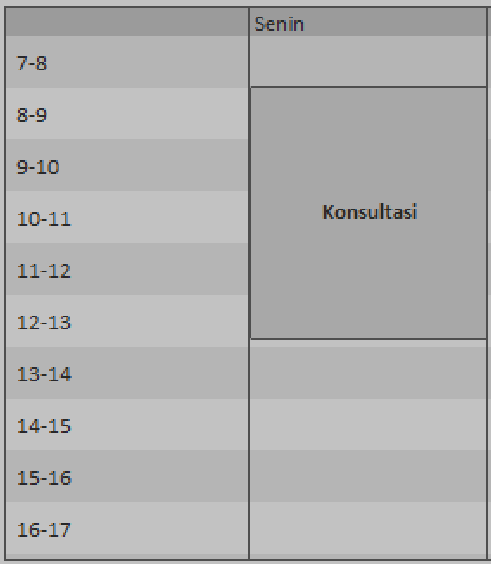
\includegraphics[scale=0.48]{contohJadwal.png}
			\caption[Contoh Jadwal]{Contoh Jadwal} 
			\label{fig:flow-chart-CodeIgniter} 
		\end{figure}
		Pada contoh diatas berarti jadwal dengan nama kegiatan "Konsultasi" yang diberi warna kuning berlangsung pada hari Senin dari jam 8 pagi sampai jam 1 siang. Warna kuning ini untuk membedakan jenis kegiatan "Konsulatsi" dengan jenis kegiatan lainnya misalnya kegiatan "Kelas" diberi warna putih. Jadwal yang ada pada tabel juga dapat ditekan untuk memunculkan menu edit yang akan dijelaskan lebih lanjut di Bagian 4.2.2 di bawah.
\end{enumerate}
\subsection{Perancangan Antarmuka Edit Jadwal Dosen}
Perancangan antarmuka untuk \textit{pop-up} yang berisi menu pengubahan data jadwal yang sudah dimasukan dapat dilihat pada gambar berikut
\begin{figure} [H]
	\centering  
	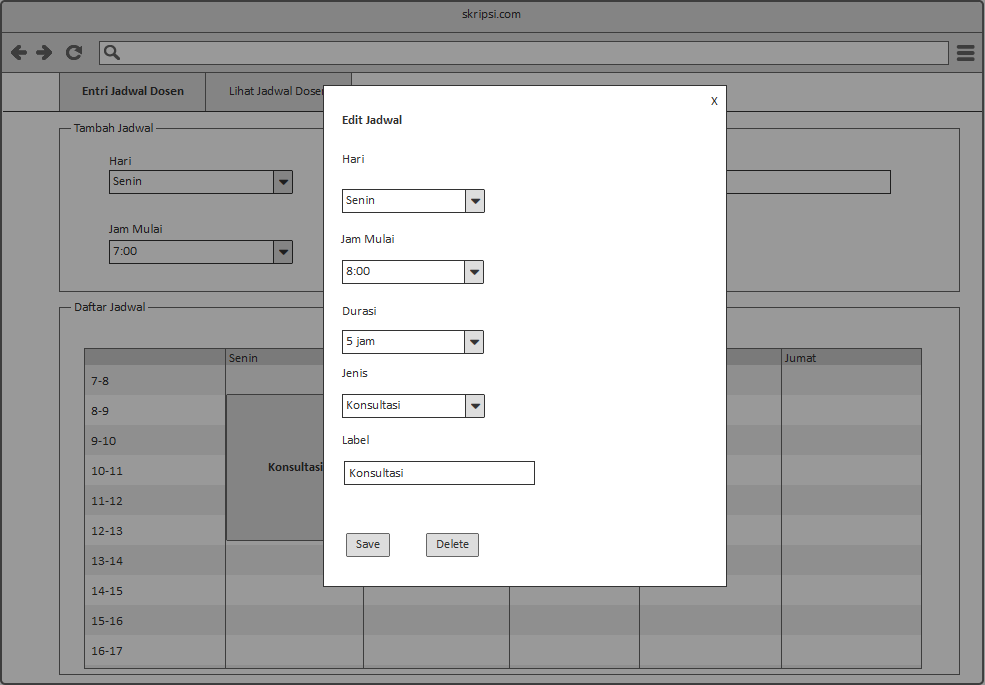
\includegraphics[scale=0.48]{editJadwalModal.png}
	\caption[Perancangan Antarmuka Edit Jadwal Dosen]{Perancangan Antarmuka Edit Jadwal Dosen} 
	\label{fig:flow-chart-CodeIgniter} 
\end{figure}
\textbf{Keterangan}
\begin{itemize}
		\item field Hari: berisi pilihan hari-hari berlangsungnya jadwal. Ada 5 pilihan hari yaitu hari senin, selasa, rabu, kamis, dan jumat.
		\item field Jam Mulai: berisi pilihan jam berlangsungnya jadwal. Jam yang dapat dipilih adalah jam 8 sampai jam 16 (jam 4 sore) dan semua 		pilihan jam tepat pada menit 0, tidak ada pilihan menitnya.
		\item field Durasi: berisi pilihan lama berlangsungnya jadwal. Ada 10 pilihan mulai dari 1 jam, 2 jam, 3 jam dan seterusnya sampai 10 			jam. Sama seperti field Jam Mulai di pilihan ini juga tidak ada pilihan menit.
		\item field Jenis: berisi pilihan jenis kegiatan jadwalnya. Ada 3 pilihan yaitu Konsultasi, Terjadwal dan Kelas.
		\item field Label: diisi dengan nama kegiatan jadwal. Field ini dapat dikosongkan.
		\item tombol Tambah: bila pengguna menekan tombol ini, maka jadwal baru akan ditambahkan sesuai dengan input yang sudah dipilih atau dimasukan oleh pengguna pada field-field di atas.
	\end{itemize}
Berdasarkan keterangan di atas menu Edit Jadwal Dosen ini sama persis dengan menu Entri Jadwal Dosen. Satu-satunya perbedaan adalah setiap \textit{field} menampilkan keterangan detil jadwal yang dipilih tersebut. Misalkan jadwal yang dipilih berlangsung dari jam 8 sampai 9, maka \textit{field} jam mulai akan menampilkan jam 8 dan \textit{field} durasi menampilkan 1 jam.

\subsection{Perancangan Antarmuka Lihat Jadwal Dosen}
Perancangan antarmuka untuk modul Lihat Jadwal Dosen dapat dilihat pada gambar di bawah ini
\begin{figure} [H]
	\centering  
	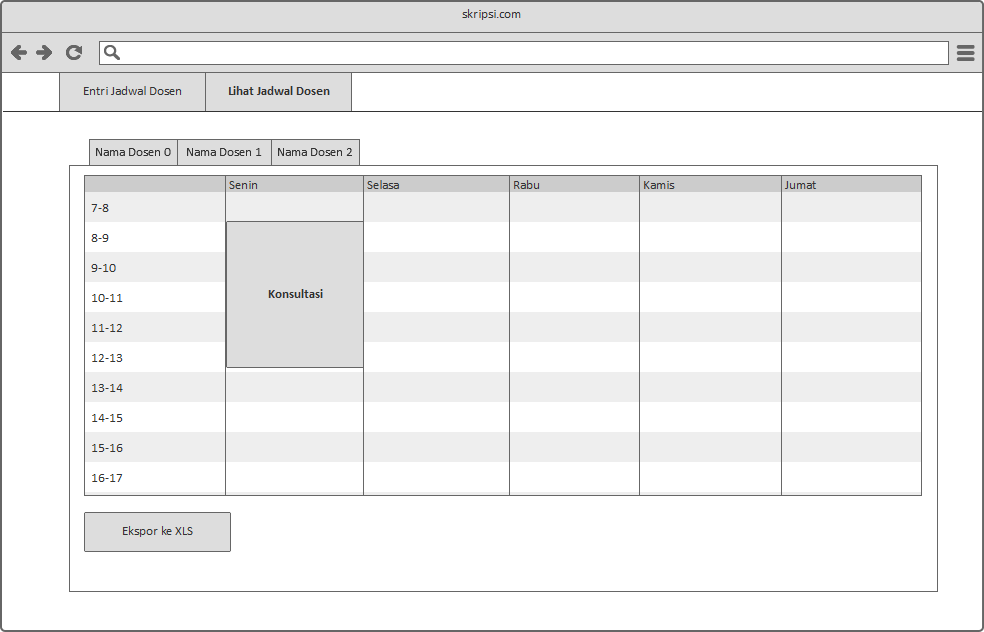
\includegraphics[scale=0.45]{lihatJadwalDosen.png}
	\caption[Perancangan Antarmuka Lihat Jadwal Dosen]{Perancangan Antarmuka Lihat Jadwal Dosen} 
	\label{fig:flow-chart-CodeIgniter} 
\end{figure}
\textbf{Keterangan}
\begin{itemize}
	\item Tab yang berlabel Nama Dosen 0, Nama Dosen 1, dan Nama Dosen 2 menandakan bahwa jadwal yang ditampilkan di tab tersebut merupakan jadwal milik dosen terkait.
	\item Tombol "Ekspor ke XLS" berfungsi untuk membuat file XLS yang berisi semua jadwal dosen yang ditampilkan di halaman Lihat Jadwal Dosen. Setiap jadwal dosen akan dikelompokan ke dalam worksheet-worksheet.
\end{itemize}
Tampilan tabel yang berisi jadwal-jadwal ini sama persis dengan tampilan di halaman Entri Jadwal Dosen, perbedaannya adalah jadwal-jadwal yang ada di dalam tabel ini tidak dapat ditekan untuk menampilkan menu Edit Jadwal Dosen.